\chapter{Turunan Asam Karboksilat}\label{ch:b2:acyl-substitution}

Didihkan minyak zaitun dengan natrium hidroksida, dan yang diperoleh adalah
sabun dan gliserol: reaksi organik tertua yang dijalankan dengan sengaja.
Minyak itu adalah ester dari gliserol dan asam-asam berantai panjang, dan
hidroksida memotong setiap ester pada satu ikatan, selalu ikatan yang sama,
yaitu antara karbon karbonil dan oksigen alkohol. Ester, asam, amida,
anhidrida, dan \omterm{def:b2:acyl-substitution:derivative}{asil klorida} semuanya bereaksi dengan cara ini: sebuah
nukleofil beradisi pada karbon karbonil, dan sebuah gugus pergi. Mengurutkan
senyawa-senyawa ini menurut seberapa mudah gugusnya pergi menunjukkan
senyawa mana yang dapat diubah menjadi senyawa mana, dan ke arah mana
seorang kimiawan harus mendaki.

\begin{recall}
Jilid Tahun 1: aktivasi elektrofilik gugus karbonil, mekanisme pembentukan
hemiasetal dan asetal, adisi organomagnesium, donor hidrida dan
jangkauannya, gugus pergi,
$\mathrm pK_a$, $Q$ dan $K$. \Cref{ch:b2:amines}: \omterm{def:b2:amines:nucleophilic-addition}{adisi nukleofilik}, amina.
\Cref{ch:b2:equilibrium-shifts}: menggeser kesetimbangan. Jilid sekolah:
ester, asam karboksilat, dan amida.
\end{recall}

\begin{omfigure}
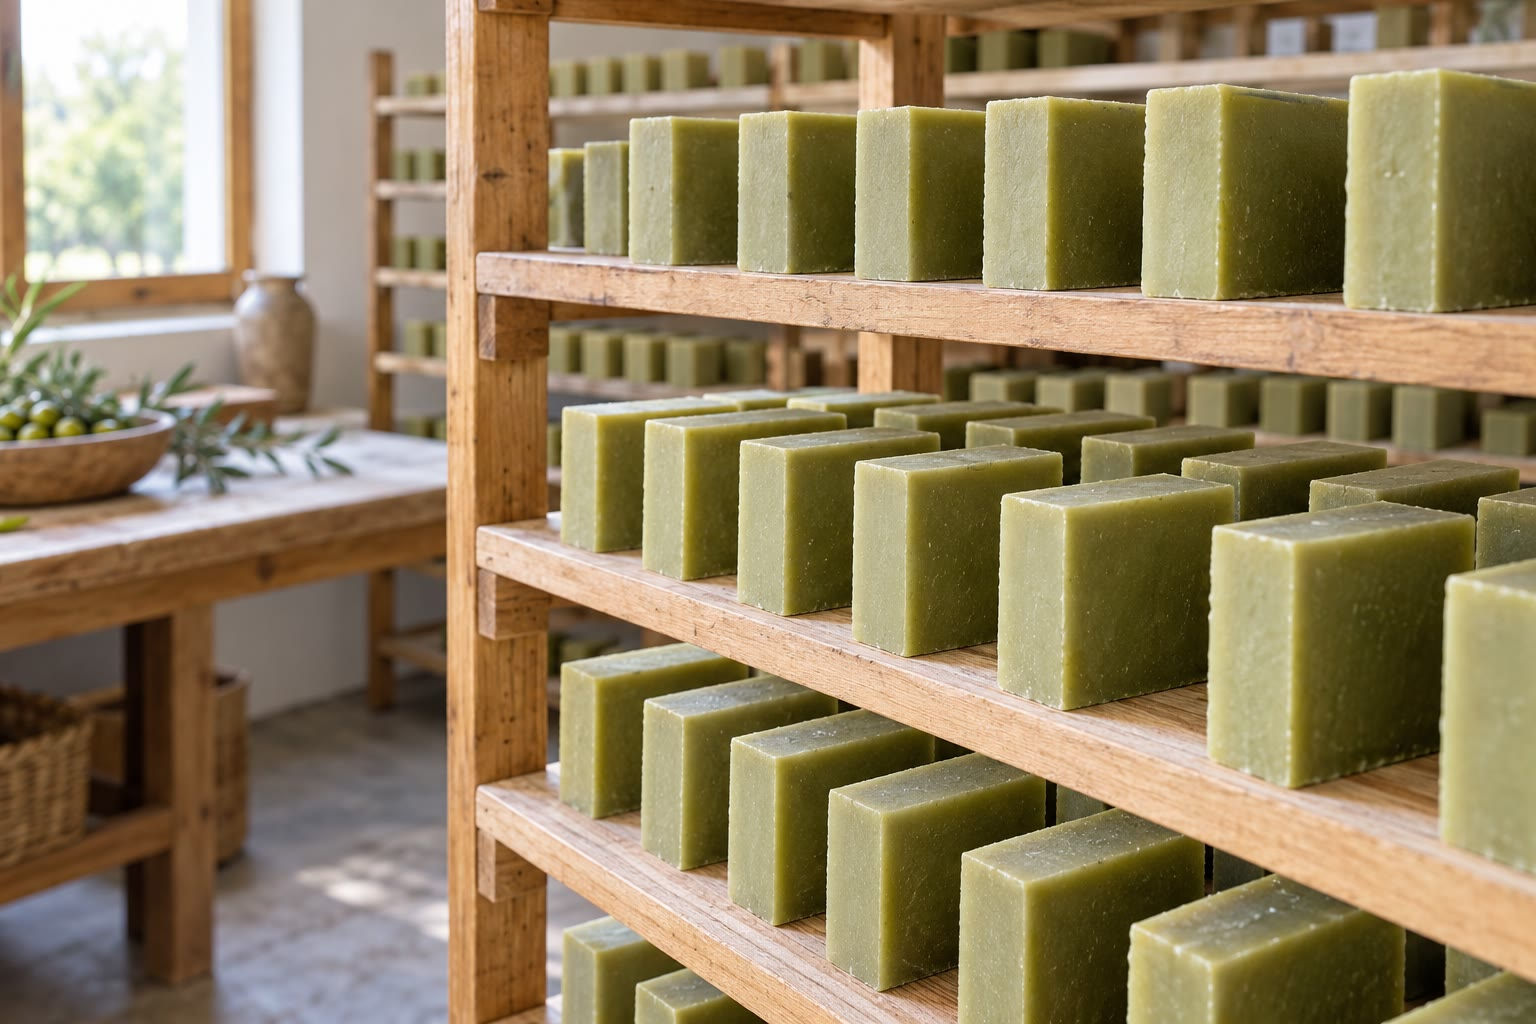
\includegraphics[width=0.58\linewidth]{images/book3/ai/b2-24-soap-bars.jpg}

{\small Batangan sabun minyak zaitun yang dikeringkan di atas rak kayu.
Sabun adalah garam natrium asam-asam lemak yang dilepaskan ketika minyak,
sebuah ester, didihkan dengan natrium hidroksida.}
\end{omfigure}

\section{Keluarga dan kereaktifannya}

\begin{definition}[Turunan asam karboksilat]\label{def:b2:acyl-substitution:derivative}
Yang disebut \emph{turunan asam karboksilat}\index{turunan asam karboksilat}
adalah senyawa \ce{R-CO-Z} yang \ce{OH} asam karboksilatnya digantikan oleh
gugus lain Z. \emph{Gugus asil}\index{gugus asil} $\mathrm{R{-}CO{-}}$ dimiliki
oleh semuanya. Dalam \emph{asil klorida}\index{asil klorida},
Z adalah Cl; dalam \emph{anhidrida asam}\index{anhidrida asam}, Z adalah
$\mathrm{O{-}CO{-}R'}$, yaitu dua gugus asil yang berbagi satu oksigen;
dalam ester Z adalah $\mathrm{OR'}$, dalam amida $\mathrm{NR'_2}$.
\end{definition}

\begin{proposition}[Skala kereaktifan]\label{prop:b2:acyl-substitution:reactivity}
Terhadap nukleofil, turunan-turunan itu bereaksi dengan urutan \omterm{def:b2:acyl-substitution:derivative}{asil klorida}
$>$ anhidrida $>$ ester $\approx$ asam $>$ amida.
\end{proposition}

\begin{proof}[Argumen]
Dua efek saling menjumlah. Gugus pergi \ce{Z-} makin mudah pergi makin lemah
kebasaannya: \ce{Cl-} (asam konjugasi \ce{HCl}, $\mathrm pK_a$ sekitar $-7$)
jauh lebih baik daripada karboksilat ($\mathrm pK_a$ sekitar 5), alkoksida
(sekitar 16), atau ion amida (sekitar 35). Selain itu, gugus Z memberikan
kerapatan elektron kepada karbonil melalui donasi mesomerik pasangan
elektron bebasnya, yang membuat karbon karbonil kurang elektrofilik: lemah
untuk Cl, paling kuat untuk nitrogen. Amida sekaligus merupakan elektrofil
terburuk dan gugus pergi terburuk.
% ledger: pka:ethanoic, pka:ethanol
\end{proof}

\section{Substitusi asil nukleofilik}

\begin{definition}[Substitusi asil nukleofilik]\label{def:b2:acyl-substitution:nas}
Yang disebut \emph{substitusi asil nukleofilik}\index{substitusi asil nukleofilik}
menggantikan gugus Z sebuah senyawa asil dengan nukleofil. Reaksi ini
berlangsung melalui adisi nukleofil pada karbon karbonil, yang menghasilkan
\emph{zat antara tetrahedral}\index{zat antara tetrahedral}, diikuti oleh
eliminasi gugus pergi, yang memulihkan ikatan \ce{C=O}.
\end{definition}

\begin{proposition}[Adisi--eliminasi]\label{prop:b2:acyl-substitution:addition-elimination}
Substitusi asil melalui \omterm{def:b2:acyl-substitution:nas}{zat antara tetrahedral}; reaksi ini dipercepat dalam
basa oleh nukleofil yang lebih kuat dan dalam asam oleh aktivasi karbonil.
\end{proposition}

\begin{proof}[Argumen]
Karbon karbonil, yang planar dan elektrofilik, menerima nukleofil dari atas
atau dari bawah bidangnya, seperti pada adisi-adisi di \cref{ch:b2:amines};
dengan gugus Z yang mampu pergi, zat antara itu mengusirnya alih-alih
terprotonasi. Dalam basa, nukleofilnya adalah anion (\ce{HO-},
\ce{RO-}); dalam asam, oksigen karbonil terprotonasi dan nukleofil netral
(air, alkohol) sudah cukup. Ester yang ditandai dengan \ce{^{18}O} pada
bagian alkoholnya menghasilkan, pada hidrolisis, alkohol bertanda dan asam
tidak bertanda: ikatan yang putus adalah ikatan asil--oksigen, sesuai dengan
tuntutan mekanismenya.
\end{proof}

\begin{omfigure}
\setchemfig{atom sep=1.7em}
\schemestart
\chemfig{R-C(=[2]O)-OR'} \+ \chemfig{HO^{-}}
\arrow{->[adisi]}
\chemfig{R-C(-[2]O^{-})(-[6]OH)-OR'}
\arrow{->[eliminasi]}[,1.3]
\chemfig{R-C(=[2]O)-OH} \+ \chemfig{^{-}OR'}
\schemestop

\medskip
\schemestart
\chemfig{R-C(=[2]O)-OH} \+ \chemfig{^{-}OR'}
\arrow{->[transfer proton]}
\chemfig{R-C(=[2]O)-O^{-}} \+ \chemfig{HOR'}
\schemestop
\par\vspace{6pt}

{\small \omterm{def:b2:acyl-substitution:saponification}{Saponifikasi} sebuah ester. Hidroksida beradisi pada karbon karbonil
dan menghasilkan \omterm{def:b2:acyl-substitution:nas}{zat antara tetrahedral}; alkoksida pergi dan ikatan \ce{C=O}
terbentuk kembali; alkoksida, sebuah basa kuat, lalu mengambil proton asam.
Tahap terakhir inilah yang membuat reaksi berlangsung tuntas.}
\end{omfigure}

\begin{method}[Menggambar substitusi asil]\label{met:b2:acyl-substitution:nas-mechanism}
\begin{enumerate}
  \item Dalam basa: nukleofil anionik beradisi pada karbon karbonil; muatan
        negatif berpindah ke oksigen; ikatan \ce{C=O} terbentuk kembali dan Z
        pergi; akhiri dengan tahap asam--basa bila ada.
  \item Dalam asam: protonasi oksigen karbonil; nukleofil netral beradisi;
        pindahkan sebuah proton ke gugus pergi; gugus itu pergi sebagai
        molekul netral; deprotonasi karbonil.
  \item Hitunglah tahap-tahapnya: setiap zat antara berupa senyawa
        tetrahedral atau senyawa karbonil.
\end{enumerate}
\end{method}

\section{Ester}

\begin{definition}[Esterifikasi]\label{def:b2:acyl-substitution:esterification}
Yang disebut \emph{esterifikasi}\index{esterifikasi} membentuk ester dari
asam karboksilat (atau turunan yang lebih reaktif) dan alkohol. Reaksi
langsung asam dengan alkohol, yang dikatalisis oleh asam kuat, adalah
esterifikasi Fischer.
\end{definition}

\begin{proposition}[Esterifikasi Fischer]\label{prop:b2:acyl-substitution:fischer}
\omterm{def:b2:acyl-substitution:esterification}{Esterifikasi} Fischer adalah kesetimbangan yang lambat, dengan tetapan
sekitar 4 untuk alkohol primer; reaksi ini didorong maju oleh kelebihan
salah satu pereaksi atau dengan mengeluarkan air begitu air terbentuk.
\end{proposition}

\begin{proof}[Argumen]
Etanol dan asam etanoat ekuimolar berhenti ketika dua pertiga asam telah
teresterifikasi: $K =
(2/3)^2/(1/3)^2 = 4$. Dengan $Q < K$ yang dipertahankan oleh kelebihan
alkohol, atau dengan menyuling air keluar (perangkap Dean--Stark dari jilid
Tahun 1), reaksi berlanjut lebih jauh
(\cref{ch:b2:equilibrium-shifts}). Keenam tahap mekanismenya adalah tahap-tahap pada \cref{met:b2:acyl-substitution:nas-mechanism}
dalam asam, semuanya reversibel.
% ledger: ester:berthelot
\end{proof}

\begin{definition}[Saponifikasi]\label{def:b2:acyl-substitution:saponification}
Yang disebut \emph{saponifikasi}\index{saponifikasi} adalah hidrolisis ester
oleh hidroksida, yang menghasilkan garam karboksilat dan alkohol.
\end{definition}

\begin{proposition}[Saponifikasi berlangsung tuntas]\label{prop:b2:acyl-substitution:saponification}
\omterm{def:b2:acyl-substitution:saponification}{Saponifikasi} berlangsung sampai tuntas: tahap terakhirnya, transfer proton
dari asam karboksilat ke alkoksida, mempunyai tetapan kesetimbangan berorde
$10^{11}$.
\end{proposition}

\begin{proof}
Untuk $\mathrm{RCOOH + R'O^- \to RCOO^- + R'OH}$,
\[
  K = \frac{K_a(\ce{RCOOH})}{K_a(\mathrm{R'OH})} = 10^{\mathrm pK_a(\mathrm{R'OH}) - \mathrm pK_a(\ce{RCOOH})} ;
\]
dengan asam etanoat (4.76) dan etanol (15.93), $K = 10^{11.2}$. Karboksilat,
elektrofil yang buruk, tidak diserang oleh alkohol: reaksi keseluruhannya
tidak berbalik.
% ledger: pka:ethanoic, pka:ethanol
\end{proof}

\begin{omfigure}
\setchemfig{atom sep=1.7em}
\schemestart
\chemfig{CH_2(-[0]O-CO-R)-[6]CH(-[0]O-CO-R)-[6]CH_2-[0]O-CO-R}
\+ \chemfig{3\,NaOH}
\arrow{->[panas]}
\chemfig{CH_2(-[0]OH)-[6]CH(-[0]OH)-[6]CH_2-[0]OH}
\+ \chemfig{3\,R-COO^{-}\,Na^{+}}
\schemestop
\par\vspace{6pt}

{\small \omterm{def:b2:acyl-substitution:saponification}{Saponifikasi} sebuah trigliserida: ketiga ikatan ester terpotong, dan
terbentuk gliserol serta tiga molekul natrium karboksilat, yaitu sabun (R
rantai panjang, \ce{C17H33} untuk oleat minyak zaitun).}
\end{omfigure}

\begin{definition}[Transesterifikasi]\label{def:b2:acyl-substitution:transesterification}
Yang disebut \emph{transesterifikasi}\index{transesterifikasi} menukar
bagian alkohol sebuah ester,
$\mathrm{RCOOR' + R''OH \rightleftharpoons RCOOR'' + R'OH}$, dengan katalisis asam atau basa.
\end{definition}

\begin{definition}[Lakton dan laktam]\label{def:b2:acyl-substitution:lactone}
Yang disebut \emph{lakton}\index{lakton} adalah ester siklik, yang terbentuk
melalui \omterm{def:b2:acyl-substitution:esterification}{esterifikasi} internal sebuah asam hidroksi; \emph{laktam}\index{laktam}
adalah amida siklik.
\end{definition}

\section{Turunan teraktivasi}

Menuruni skala kereaktifan itu mudah: \omterm{def:b2:acyl-substitution:derivative}{asil klorida} menghasilkan anhidrida,
ester, atau amida dengan nukleofil yang tepat, sering pada suhu kamar.
Mendakinya memerlukan aktivasi: asam karboksilat diubah menjadi kloridanya
oleh tionil klorida,
\[
  \ce{RCOOH + SOCl2 -> RCOCl + SO2 + HCl} ,
\]
yang produk-produk sampingnya berupa gas. \omterm{def:b2:acyl-substitution:derivative}{Asil klorida} lalu bereaksi dengan
alkohol atau amina; sebuah basa (piridina, trietilamina, atau ekuivalen
kedua amina itu) menangkap \ce{HCl} yang terbentuk, yang jika tidak
demikian akan memprotonasi amina.

\begin{method}[Berpindah di antara turunan-turunan]\label{met:b2:acyl-substitution:ladder}
\begin{enumerate}
  \item Menuruni skala (klorida $\to$ anhidrida $\to$ ester, asam $\to$ amida):
        reaksikan dengan nukleofil, bersama basa untuk mengikat asam yang
        dilepaskan.
  \item Mendaki skala: ubahlah asam menjadi klorida lebih dahulu
        (\ce{SOCl2}); ester atau amida dihidrolisis menjadi asam lebih dahulu.
  \item Di antara asam dan ester: \omterm{def:b2:acyl-substitution:esterification}{esterifikasi} Fischer (kesetimbangan) atau
        \omterm{def:b2:acyl-substitution:saponification}{saponifikasi} (tuntas) yang diikuti oleh pengasaman.
\end{enumerate}
\end{method}

\begin{omfigure}
\begin{tikzpicture}[font=\small, >={Stealth}]
  \foreach \y/\n in {4/{asil klorida \ce{RCOCl}}, 3/{anhidrida \ce{(RCO)2O}}, 2/{ester $\mathrm{RCOOR'}$ \quad asam \ce{RCOOH}}, 1/{amida $\mathrm{RCONR'_2}$}} {
    \node[cyclenode, minimum width=5.2cm] at (0,\y*1.1) {\n};
  }
  \draw[->, thick, omDef] (-3.1,4.3) -- (-3.1,1.1) node[midway, left, align=right, font=\scriptsize] {mudah:\\ nukleofil\\ + basa};
  \draw[->, thick, omThm] (3.1,2.2) -- (3.1,4.4) node[midway, right, align=left, font=\scriptsize] {mendaki:\\ melalui asam\\ dan \ce{SOCl2}};
  \node[font=\scriptsize, anchor=south] at (0,4.85) {lebih reaktif};
  \node[font=\scriptsize, anchor=north] at (0,0.55) {kurang reaktif};
\end{tikzpicture}

{\small Tangga kereaktifan \omterm{def:b2:acyl-substitution:derivative}{turunan asam karboksilat}. Setiap turunan dapat
diubah menjadi turunan di bawahnya oleh nukleofil; mendaki harus melalui
asam dan kloridanya.}
\end{omfigure}

\section{Organologam dan hidrida}

\begin{proposition}[Dua adisi Grignard]\label{prop:b2:acyl-substitution:grignard-ester}
Ester yang direaksikan dengan pereaksi organomagnesium berlebih menghasilkan
alkohol tersier yang membawa dua gugus identik dari pereaksi itu.
\end{proposition}

\begin{proof}[Argumen]
Adisi pertama menghasilkan \omterm{def:b2:acyl-substitution:nas}{zat antara tetrahedral} yang mengusir alkoksida:
sebuah keton. Keton lebih elektrofilik daripada ester (tidak ada donasi
mesomerik dari gugus $\mathrm{OR'}$) dan bereaksi dengan pereaksi itu lebih
cepat daripada ester yang tersisa; adisi kedua, pada keton, menghasilkan
alkoksida alkohol tersier, yang diprotonasi pada pengolahan asam. Reaksi itu
tidak dapat dihentikan pada keton.
\end{proof}

\begin{proposition}[Reduksi hidrida]\label{prop:b2:acyl-substitution:hydrides}
Litium aluminium hidrida mereduksi ester dan asam menjadi alkohol primer,
dan amida menjadi amina; natrium borohidrida mereduksi aldehida dan keton
tetapi tidak mereduksi ester, asam, atau amida. Aluminium hidrida yang
meruah (DIBAL-H) pada \qty{-78}{\degreeCelsius} mereduksi ester menjadi
aldehida.
\end{proposition}

\begin{proof}[Argumen]
\ce{LiAlH4} adalah donor hidrida yang kuat: seperti pereaksi Grignard,
senyawa ini beradisi dua kali pada ester (melalui aldehida). Borohidrida
terlalu lemah untuk karbonil ester yang kurang elektrofilik. Dengan DIBAL-H
pada suhu rendah, \omterm{def:b2:acyl-substitution:nas}{zat antara tetrahedral}, yang ditahan oleh aluminium, tidak
mengusir alkoksida sampai pengolahan berair, ketika tidak ada lagi hidrida
yang tersisa: aldehidanya bertahan. Pada amida, oksigen yang terikat pada
aluminium yang dieliminasi alih-alih nitrogen, sehingga tersisa ion iminium
yang direduksi oleh hidrida menjadi amina.
\end{proof}

\begin{history}[Chevreul dan lemak]
\begin{minipage}[t]{0.22\linewidth}
\vspace{0pt}
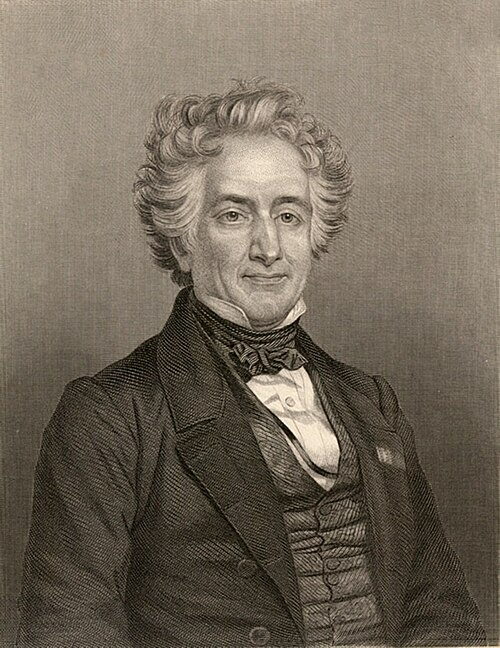
\includegraphics[width=\linewidth]{images/book3/chevreul.jpg}
\end{minipage}\hfill
\begin{minipage}[t]{0.74\linewidth}
\vspace{0pt}
Michel Eugène Chevreul menunjukkan, dalam sebuah kajian yang diterbitkan
pada tahun 1823, bahwa lemak adalah senyawa gliserol dengan asam-asam lemak,
yang ia isolasi dan namai (asam stearat, oleat, butirat), dan bahwa
\omterm{def:b2:acyl-substitution:saponification}{saponifikasi} memecahnya menjadi kedua bagian itu. Karyanya mengubah
pembuatan sabun dan lilin menjadi kimia; ia hidup sampai usia 102 tahun.
(Potret oleh Nicolas Eustache Maurin, domain publik, Wikimedia
Commons.)
\end{minipage}
\end{history}

\begin{safety}{\ghs[5mm]{GHS02}\,\ghs[5mm]{GHS05}\,\ghs[5mm]{GHS06}}
Tionil klorida dan \omterm{def:b2:acyl-substitution:derivative}{asil klorida} bereaksi hebat dengan air dan melepaskan gas
korosif; senyawa-senyawa itu ditangani dalam keadaan kering, di dalam lemari
asam. Litium aluminium hidrida menyala jika bersentuhan dengan air;
kelebihannya dimusnahkan dengan hati-hati di akhir. Natrium hidroksida pekat
korosif terhadap kulit dan mata. Metanol beracun dan mudah terbakar.
% ledger: ghs:SOCl2, ghs:ethanoyl-chloride, ghs:LiAlH4, ghs:NaOH, ghs:methanol
\end{safety}

\section{Latihan}

\begin{exercise}[$\star$]\label{exo:b2:acyl-substitution:1}
Urutkan menurut kereaktifan terhadap air: etil etanoat, etanoil klorida,
etanamida, anhidrida etanoat.
\end{exercise}

\begin{exercise}[$\star$]\label{exo:b2:acyl-substitution:2}
Tuliskan produk-produk etanoil klorida dengan: air; etanol; amonia (2
ekuivalen); natrium etanoat; dimetilamina dengan trietilamina.
\end{exercise}

\begin{exercise}[$\star$]\label{exo:b2:acyl-substitution:3}
Tuliskan \omterm{def:b2:acyl-substitution:saponification}{saponifikasi} metil benzoat oleh natrium hidroksida dan hitunglah
massa natrium hidroksida yang diperlukan untuk \qty{13.6}{g} ester itu.
\end{exercise}

\begin{exercise}[$\star$]\label{exo:b2:acyl-substitution:4}
Gambarlah \omterm{def:b2:acyl-substitution:lactone}{lakton} yang dibentuk oleh asam 4-hidroksibutanoat dan tentukan ukuran cincinnya.
\end{exercise}

\begin{exercise}[$\star\star$]\label{exo:b2:acyl-substitution:5}
Tuliskan mekanisme reaksi etil etanoat dengan amonia.
\end{exercise}

\begin{exercise}[$\star\star$]\label{exo:b2:acyl-substitution:6}
Aspirin dibuat dari asam salisilat (asam 2-hidroksibenzoat) dan anhidrida
etanoat. Gugus asam salisilat manakah yang bereaksi, dan apa produk
sampingnya?
\end{exercise}

\begin{exercise}[$\star\star$]\label{exo:b2:acyl-substitution:7}
Etil etanoat direaksikan dengan metilmagnesium bromida berlebih, lalu dengan
asam encer. Tuliskan produknya dan jelaskan mengapa ketonnya tidak dapat
diisolasi.
\end{exercise}

\begin{exercise}[$\star\star$]\label{exo:b2:acyl-substitution:8}
Tuliskan produk reduksi \omterm{def:b2:acyl-substitution:lactone}{lakton} pada latihan 4 oleh \ce{LiAlH4}.
\end{exercise}

\begin{exercise}[$\star\star$]\label{exo:b2:acyl-substitution:9}
Dengan $K = 4$, hitunglah fraksi asam etanoat yang teresterifikasi dengan
satu, lalu dengan tiga ekuivalen etanol. Metode lain apakah yang mendorong
reaksi itu?
\end{exercise}

\begin{exercise}[$\star\star\star$]\label{exo:b2:acyl-substitution:10}
Buatlah \textit{N},\textit{N}-dietilbenzamida dari asam benzoat, dan
jelaskan mengapa mencampur asam itu dengan dietilamina dan memanaskannya
secara lunak justru menghasilkan garam.
\end{exercise}

\begin{exercise}[$\star\star\star$]\label{exo:b2:acyl-substitution:11}
Bilangan penyabunan sebuah lemak adalah massa kalium hidroksida, dalam mg,
yang diperlukan untuk menyabunkan \qty{1}{g} lemak itu. Hitunglah bilangan
itu untuk triolein (\qty{885.4}{g/mol}; KOH \qty{56.11}{g/mol}).
\end{exercise}

\begin{exercise}[$\star\star\star$]\label{exo:b2:acyl-substitution:12}
Sebuah molekul membawa ester, amida, dan keton. Gugus mana yang direduksi
oleh \ce{NaBH4}, dan mana yang oleh \ce{LiAlH4}? Apa yang diperoleh dalam
setiap kasus?
\end{exercise}

\section{Soal: Biodiesel dari Minyak Goreng}

\begin{problem}[{Soal akhir pekan --- triolein dan massa molarnya,
transesterifikasinya dengan metanol dan peran basa, reaksi samping dengan
asam bebas dan air, serta rendemen per ton minyak}]
\label{pb:b2:acyl-substitution:1}
Modelkan minyak itu sebagai triolein murni, trigliserida asam oleat
(\ce{C17H33COOH}). Massa molar
(\unit{g/mol}): C 12.011, H 1.008, O 15.999, Na 22.990. Gliserol adalah
propana-1,2,3-triol.
% ledger: aw:C, aw:H, aw:O, aw:Na, ghs:methanol, ghs:NaOH

\medskip
\noindent\textbf{Bagian I --- Triolein.}
\begin{enumerate}
  \item Tuliskan rumus asam oleat dan gliserol.
  \item Tuliskan rumus triolein dan hitunglah massa molarnya.
  \item Berapa gugus ester yang dikandungnya?
  \item Asam oleat mempunyai satu ikatan rangkap cis. Mengapa minyak yang
        kaya akan asam ini berwujud cair pada suhu kamar?
  \item Apa yang akan dihasilkan oleh \omterm{def:b2:acyl-substitution:saponification}{saponifikasi} triolein?
  \item Secara kimia, apakah biodiesel itu?
\end{enumerate}

\medskip
\noindent\textbf{Bagian II --- \omterm{def:b2:acyl-substitution:transesterification}{Transesterifikasi}.}
\begin{enumerate}[resume]
  \item Tuliskan \omterm{def:b2:acyl-substitution:transesterification}{transesterifikasi} triolein dengan metanol.
  \item Mengapa basa (natrium metoksida atau hidroksida) dipakai sebagai katalis?
  \item Gambarlah \omterm{def:b2:acyl-substitution:nas}{zat antara tetrahedral} pada pertukaran pertama.
  \item Mengapa metanol dipakai berlebih (enam ekuivalen alih-alih tiga)?
  \item Gliserol tidak dapat bercampur dengan metil ester. Bagaimana hal ini membantu?
  \item Apakah katalis terpakai dalam reaksi ideal?
\end{enumerate}

\medskip
\noindent\textbf{Bagian III --- Asam bebas dan air.}
\begin{enumerate}[resume]
  \item Minyak goreng bekas mengandung asam oleat bebas. Apa pengaruhnya terhadap basa?
  \item Apa pengaruh air terhadap metil ester dengan adanya basa?
  \item Mengapa sabun yang terbentuk mengganggu?
  \item Bagaimana asam-asam bebas itu dapat disingkirkan lebih dahulu, tanpa basa?
  \item Mengapa minyak harus dikeringkan sebelum reaksi?
\end{enumerate}

\medskip
\noindent\textbf{Bagian IV --- Per ton minyak.}
\begin{enumerate}[resume]
  \item Hitunglah jumlah triolein dalam satu ton.
  \item Hitunglah massa metanol yang terpakai.
  \item Hitunglah massa metil oleat yang terbentuk.
  \item Periksalah kekekalan massa.
  \item Sebuah minyak dengan 2~\% massa asam oleat bebas direaksikan dengan
        natrium hidroksida: hitunglah massa natrium hidroksida yang terpakai
        oleh asam itu per ton.
  \item Hitunglah massa gliserol yang ikut dihasilkan per ton triolein.
\end{enumerate}
\end{problem}
